% !TeX program = lualatex
% ================================================================
% Polish Tier 3 Vocabulary Version of CollectingAndMultiplyingTerms
%
% Generated by the server using the following settings:
%
%   language            Polish (pol)
%   text direction      left to right
%   font                Noto Serif
%   fallback font       Noto Serif
%   built from          latex/worksheets/algebra/collectingAndMultiplyingTerms.tex
%   vocabulary key      latex/worksheets/algebra/collectingAndMultiplyingTerms/L2/pol/collectingAndMultiplyingTerms_polishKey.tex
%   tier 3 vocabulary   green   RGB 0 128 0
%   English text        black   RGB 0 0 0
%   Polish text         purple  RGB 112 48 160
%   layout macros       version 3
%
% Please don't edit any information in this comment block - the server
% compares it against the current settings and rebuilds this file when
% they differ, so changes here would be overwritten. However, feel free
% to make updates to the LaTeX below if you want to edit it.
% ================================================================

\documentclass[12pt,a4paper]{article}
% ================================================================
% Copied from the English sheet this was translated from, so that
% anything it sets up for itself still works here
% ================================================================
\usepackage[a4paper,top=12mm,bottom=12mm,left=14mm,right=14mm]{geometry}
\usepackage[T1]{fontenc}
\usepackage{amsmath}
\usepackage{amssymb}
% A sans serif font with a single-storey a, as children write it. It is
% used for the mathematics as well as the text.
\usepackage{tgadventor}
\renewcommand*{\familydefault}{\sfdefault}
\usepackage[italic]{mathastext}
\usepackage{multicol}
\usepackage{tikz}
\usepackage[most]{tcolorbox}
\usetikzlibrary{arrows.meta}

% ================================================================
% Collecting and multiplying terms: a drill booklet that follows the
% algebraic terminology sheet.
%
% Each page practises one kind of simplification, and each page is a
% small step on from the one before:
%
%   1  adding terms in one variable
%   2  subtracting terms in one variable
%   3  collecting like terms, all positive
%   4  collecting like terms with subtraction (the sign belongs to
%      the term)
%   5  collecting like terms where a coefficient comes out negative
%   6  multiplying terms
%   7  multiplying terms with negative coefficients
%   8  multiplying a variable by itself: squares and cubes
%   9  multiplying powers of one variable
%  10  multiplying powers of more than one variable
%  11  collecting like terms with powers
%  12  multiplying, then collecting like terms
%  13  problem solving
%
% Pages 1 to 12 have the same three parts. A worked example shows the
% method, with a note beside it saying why it works. Then two questions
% repeat the worked example's layout line for line, the first with
% most of the working given and the second with only the words given,
% so that the support is taken away in two steps. Then there is a list
% of questions in two columns that starts easier than the worked
% example and finishes a little harder.
%
% The answers are in a comment beside each question.
% ================================================================

\pagestyle{empty}
\setlength{\parindent}{0pt}
\setlength{\parskip}{0pt}
\setlength{\columnsep}{8mm}
\setlength{\multicolsep}{4pt}
% Ragged right, so that the spaces between words are all the same.
\AtBeginDocument{\raggedright}

% The worked examples and the key idea, in boxes that are tinted only
% faintly, so that the sheet is cheap to print.
\newtcolorbox{keyidea}{colback=orange!3,colframe=orange!35,boxrule=0.6pt,
  left=6pt,right=6pt,top=4pt,bottom=4pt,before upper=\raggedright}
\newtcolorbox{wex}{colback=blue!2,colframe=blue!30,boxrule=0.6pt,
  colbacktitle=blue!8,coltitle=blue!50!black,
  left=6pt,right=6pt,top=2pt,bottom=4pt,before upper=\raggedright,
  title={\bfseries Worked example},toptitle=1pt,bottomtitle=1pt}

% The title of a page. The questions are numbered from 1 again on each
% page, so that a question can be found from its page and its number.
\newcommand{\topic}[1]{\setcounter{qnum}{0}{\Large\bfseries #1}\par\vspace{6pt}}

% An instruction for the questions after it.
\newcommand{\instruction}[1]{\par\vspace{10pt}{\bfseries #1}\par\vspace{2pt}}

% Gaps to write in: \gap for a term, \wgap for a longer term or a short
% expression, and \lgap for a long expression. The strut keeps the
% lines far enough apart to write on.
\newcommand{\gapstrut}{\rule[-1.8mm]{0pt}{8mm}}
\newcommand{\gap}{\gapstrut\underline{\hspace{1.5cm}}}
\newcommand{\wgap}{\gapstrut\underline{\hspace{2.6cm}}}
\newcommand{\lgap}{\gapstrut\underline{\hspace{4.2cm}}}
% A gap for an index. An underline sits too low to be read as an index,
% so a faint dotted box marks where the number is written.
\newcommand{\boxgap}{\tikz[baseline=-0.8pt]\draw[gray!60,densely dotted,thick]
  (0,0) rectangle (8pt,8pt);}

% The method, set out one line at a time. The worked example and the
% two questions after it all use this width, so that their lines break
% in the same places and the layouts match line for line.
\newlength{\workwidth}\setlength{\workwidth}{7.7cm}
\newlength{\qlabelwidth}\setlength{\qlabelwidth}{1.1cm}
\newenvironment{working}
  {\begin{minipage}[t]{\workwidth}\raggedright\everypar{\gapstrut}}
  {\end{minipage}}
% The note beside the working, in the rest of the worked example box.
\newenvironment{wexnote}
  {\hfill\begin{minipage}[t]{\dimexpr\linewidth-\workwidth-6mm\relax}%
   \raggedright\vspace{4pt}\setlength{\parskip}{5pt}}
  {\end{minipage}}

% The question number. A question that runs onto a second line is
% indented to line up with its first line.
\newcounter{qnum}
\newcommand{\qlabel}{\stepcounter{qnum}\hangindent=\qlabelwidth\hangafter=1
  \makebox[\qlabelwidth][l]{\textbf{Q\theqnum.}}}

% A question that repeats the worked example with gaps in it. Two of
% them sit side by side.
\newenvironment{scaffold}
  {\begin{minipage}[t]{0.49\linewidth}\qlabel\begin{working}}
  {\end{working}\end{minipage}}

% The list of questions, in two columns. Each question is a term or an
% expression to simplify, then an answer line to the end of the column.
% \sq is for a short question, and \sql puts the answer line on a line
% of its own, for a long one. (TeX removes glue from the end of a
% paragraph, so a \kern follows the line to keep it.)
\newenvironment{questions}
  {\begin{multicols}{2}\raggedright}
  {\end{multicols}}
\newcommand{\ansline}{\nobreak\hspace{2pt}\gapstrut
  \leaders\hrule\hskip 2.8cm plus 1fill\kern0pt\par}
\newcommand{\sq}[1]{\par\qlabel$#1={}$\ansline\vspace{7pt}}
\newcommand{\sql}[1]{\par\qlabel$#1$\par
  \hspace*{\qlabelwidth}$={}$\ansline\vspace{7pt}}

% A line to write a sentence on, the width of the column.
\newcommand{\writeline}{\par\gapstrut\leaders\hrule\hskip 0pt plus 1fill\kern0pt\par}

% A box for a missing term.
\newcommand{\missing}{\tikz[baseline=-4pt]\draw[thick] (0,-0.25) rectangle (1.5,0.55);}

% Characters this language's font has not got are borrowed from another,
% rather than being silently dropped - see docs/translated-sheet-latex.md
\directlua{%
  if luaotfload and luaotfload.add_fallback then
    luaotfload.add_fallback("eallatinfallback",
      { "Noto Serif:mode=harf;" })
  else
    tex.error("this luaotfload is too old to register a fallback font")
  end
}
\usepackage[english]{babel}
\babelprovide[import]{polish}
\babelfont[polish]{rm}[Renderer=Harfbuzz, BoldFont={Noto Serif}, ItalicFont={Noto Serif}, BoldItalicFont={Noto Serif}, RawFeature={fallback=eallatinfallback}]{Noto Serif}
\babelfont[polish]{sf}[Renderer=Harfbuzz, BoldFont={Noto Serif}, ItalicFont={Noto Serif}, BoldItalicFont={Noto Serif}, RawFeature={fallback=eallatinfallback}]{Noto Serif}
\newcommand{\ealtext}[1]{\foreignlanguage{polish}{#1}}
\newcommand{\ealtextblock}[1]{{\raggedright\foreignlanguage{polish}{#1}\par}}
% ================================================================
% EAL layout helpers
% ================================================================
\usepackage{xcolor}

\definecolor{ealkeycolour}{RGB}{0,128,0}
\definecolor{ealenglish}{RGB}{0,0,0}
\definecolor{ealtwocolour}{RGB}{112,48,160}

\newsavebox{\ealboxen}
\newsavebox{\ealboxtr}
\newlength{\ealglosswd}
\newlength{\ealglossraise}
\setlength{\ealglossraise}{1.15em}

% a tier 3 word, in English and in translation alike
\newcommand{\ealkey}[1]{\textcolor{ealkeycolour}{#1}}
\newcommand{\ealkeytr}[1]{\textcolor{ealkeycolour}{\ealtext{#1}}}

% One translated word above one English word. Built from kernel
% primitives, never a tabular, which would break wherever the sheet
% loads array, booktabs or tabularx. The box is as wide as the wider of
% the two, so a long translation pushes its neighbours aside instead of
% overlapping them, and it claims its full height so a table row or a
% TikZ node makes room for it.
\newcommand{\ealgloss}[2]{%
  \sbox{\ealboxen}{\ealkey{#1}}%
  \sbox{\ealboxtr}{\small\textcolor{ealtwocolour}{\ealtext{#2}}}%
  \setlength{\ealglosswd}{\wd\ealboxen}%
  \ifdim\wd\ealboxtr>\ealglosswd\setlength{\ealglosswd}{\wd\ealboxtr}\fi
  \leavevmode
  \makebox[\ealglosswd][c]{%
    \makebox[0pt][c]{\usebox{\ealboxen}}%
    \makebox[0pt][c]{\raisebox{\ealglossraise}{\usebox{\ealboxtr}}}%
  }%
}

% opens up line spacing around a block of glosses, so the raised
% translations sit clear of the line above
\newenvironment{ealglossed}{\par\linespread{2.1}\selectfont\ignorespaces}{\par}

% a whole translated sentence above its English counterpart. block level,
% so it does not belong inside a tabular cell
\newcommand{\ealpara}[2]{%
  \par\addvspace{0.5\baselineskip}%
  {\color{ealtwocolour}\ealtextblock{#1}}%
  \penalty200
  {\color{ealenglish}#2\par}%
  \addvspace{0.5\baselineskip}%
}

\begin{document}
\begin{ealglossed}

\begin{center}
  {\LARGE\bfseries \ealgloss{Collecting}{redukowanie} and Multiplying \ealgloss{Terms}{wyrazy}}
\end{center}
\vspace{-6pt}

\begin{keyidea}
A \ealgloss{term}{wyraz} is a number, a \ealgloss{variable}{zmienna}, or numbers and \ealgloss{variables}{zmienne}
multiplied together. The \ealgloss{coefficient}{współczynnik} of a \ealgloss{term}{wyraz} is the number that
multiplies the \ealgloss{variables}{zmienne} in it.

\vspace{3pt}
To \ealgloss{simplify}{uprościć} an \ealgloss{expression}{wyrażenie}, we write it in a shorter way that is
equal to it for every value of the \ealgloss{variables}{zmienne}. Follow the worked examples in
this booklet to learn how to \ealgloss{simplify}{uprościć} \ealgloss{expressions}{wyrażenia}.
\end{keyidea}

\vspace{6pt}
\topic{1. Adding \ealgloss{terms}{wyrazy}}

\begin{wex}
\begin{working}
\ealgloss{Simplify}{Uprość} $3a+2a$.

$3a$ means $a+a+a$.

$2a$ means $a+a$.

$3a+2a=a+a+a+a+a$

So $3a+2a=5a$.
\end{working}
\begin{wexnote}
$3a$ means $3\times a$, which is $a+a+a$. The \ealgloss{coefficient}{współczynnik} of $3a$ is $3$.

In $3a+2a$, the \ealgloss{variable}{zmienna} $a$ is added $3+2=5$ times. So to add the \ealgloss{terms}{wyrazy},
we add their \ealgloss{coefficients}{współczynniki}.

A \ealgloss{variable}{zmienna} on its own has a \ealgloss{coefficient}{współczynnik} of $1$: $b$ means $1b$. So
$b+2b=3b$. We write $b$, not $1b$.
\end{wexnote}
\end{wex}

\instruction{Fill in the gaps.}

\begin{scaffold}
\ealgloss{Simplify}{Uprość} $4b+3b$.

$4b$ means $b+b+b+b$.

$3b$ means \wgap.

$4b+3b=b+b+b+b+b+b+b$

So $4b+3b=$ \gap.
\end{scaffold}\hfill
\begin{scaffold}
\ealgloss{Simplify}{Uprość} $2x+5x$.

$2x$ means \wgap.

$5x$ means \lgap.

$2x+5x=$ \lgap

So $2x+5x=$ \gap.
\end{scaffold}

\instruction{\ealgloss{Simplify}{Uprość}.}

\begin{questions}
\sq{5a+2a}
\sq{3b+4b}
\sq{6x+3x}
\sq{2y+8y}
\sq{4m+4m}
\sq{7p+5p}
\sq{a+4a}
\sq{9t+t}
\sq{c+c}
\sq{10n+6n}
\sq{2a+3a+4a}
\sq{5k+k+6k}
\sq{x+x+x+x}
\sq{12y+15y}
\sq{3d+2d+d+4d}
\sq{20z+13z+7z}
\end{questions}

\newpage

\topic{2. Subtracting \ealgloss{terms}{wyrazy}}

\begin{wex}
\begin{working}
\ealgloss{Simplify}{Uprość} $8a+3a-5a$.

We work from left to right.

$8a+3a=11a$

$11a-5a=6a$

So $8a+3a-5a=6a$.
\end{working}
\begin{wexnote}
To subtract \ealgloss{terms}{wyrazy} with the same \ealgloss{variable}{zmienna}, we subtract their \ealgloss{coefficients}{współczynniki}:
$11-5=6$.

When there are more than two \ealgloss{terms}{wyrazy}, we work from left to right, one \ealgloss{term}{wyraz}
at a time.

When the \ealgloss{coefficient}{współczynnik} is $1$, we write $a$, not $1a$. When the \ealgloss{coefficients}{współczynniki}
\ealgloss{cancel out}{skrócić się}, the answer is $0$: $4a-4a=0$.
\end{wexnote}
\end{wex}

\instruction{Fill in the gaps.}

\begin{scaffold}
\ealgloss{Simplify}{Uprość} $6b+4b-3b$.

We work from left to right.

$6b+4b=10b$

$10b-3b=$ \gap

So $6b+4b-3b=$ \gap.
\end{scaffold}\hfill
\begin{scaffold}
\ealgloss{Simplify}{Uprość} $9x-2x+5x$.

We work from left to right.

$9x-2x=$ \gap

\gap\ $+\,5x=$ \gap

So $9x-2x+5x=$ \gap.
\end{scaffold}

\instruction{\ealgloss{Simplify}{Uprość}.}

\begin{questions}
\sq{7a-3a}
\sq{9b-4b}
\sq{10x-6x}
\sq{8y-y}
\sq{12m-5m}
\sq{14q-8q}
\sq{11h-h}
\sq{5p-4p}
\sq{6t-6t}
\sq{20n-9n}
\sq{25w-17w}
\sq{4a+6a-3a}
\sq{5k+k-2k}
\sq{9a+a-4a}
\sq{8b+2b-7b}
\sq{9p-2p+4p}
\sq{6r-4r+5r}
\sq{12t-5t-2t}
\sq{10g-3g-3g}
\sq{x+7x-3x}
\sq{10c-4c-6c}
\sq{8y-3y+2y-4y}
\sq{7m+m-5m+2m}
\sq{15d-7d+d-8d}
\end{questions}

\newpage

\topic{3. \ealgloss{Collecting}{redukowanie} \ealgloss{like terms}{wyrazy podobne}}

\begin{wex}
\begin{working}
\ealgloss{Simplify}{Uprość} $5a+3b+2a+4b$.

The \ealgloss{like terms}{wyrazy podobne} are $5a$ and $2a$, and $3b$ and $4b$.

$5a+2a=7a$

$3b+4b=7b$

So $5a+3b+2a+4b=7a+7b$.
\end{working}
\begin{wexnote}
\ealgloss{Like terms}{wyrazy podobne} have exactly the same \ealgloss{variables}{zmienne}. $5a$ and $2a$ are \ealgloss{like terms}{wyrazy podobne},
and $3b$ and $4b$ are \ealgloss{like terms}{wyrazy podobne}.

We \ealgloss{collect}{redukujemy} each set of \ealgloss{like terms}{wyrazy podobne} into a single \ealgloss{term}{wyraz}.

$7a$ and $7b$ are not \ealgloss{like terms}{wyrazy podobne}, so $7a+7b$ cannot be \ealgloss{simplified}{uprościć}.

\ealgloss{Constants}{stałe} are \ealgloss{like terms}{wyrazy podobne} with each other: $4+2=6$.
\end{wexnote}
\end{wex}

\instruction{Fill in the gaps.}

\begin{scaffold}
\ealgloss{Simplify}{Uprość} $4x+2y+3x+5y$.

The \ealgloss{like terms}{wyrazy podobne} are $4x$ and $3x$, and \gap\ and \gap.

$4x+3x=$ \gap

$2y+5y=$ \gap

So $4x+2y+3x+5y=$ \wgap.
\end{scaffold}\hfill
\begin{scaffold}
\ealgloss{Simplify}{Uprość} $2m+6n+m+3n$.

The \ealgloss{like terms}{wyrazy podobne} are \gap\ and \gap, and \gap\ and \gap.

\gap\ $+$ \gap\ $=$ \gap

\gap\ $+$ \gap\ $=$ \gap

So $2m+6n+m+3n=$ \wgap.
\end{scaffold}

\instruction{\ealgloss{Simplify}{Uprość}. If an \ealgloss{expression}{wyrażenie} cannot be \ealgloss{simplified}{uprościć}, write
``cannot be \ealgloss{simplified}{uprościć}''.}

\begin{questions}
\sq{3a+2b+4a}
\sq{5x+2y+3y}
\sq{4p+3p+2q}
\sq{2x+3x+4y}
\sq{2a+3b+4a+b}
\sq{6p+q+2p+5q}
\sq{3m+4n+3m+4n}
\sq{4a+5+3a}
\sq{x+4+3x+2}
\sq{6+3t+t}
\sq{7+2m+5+m}
\sq{4m+n+2+m}
\sq{5y+1+y+8}
\sq{3a+2b+6}
\sq{a+b+a+b+a}
\sql{4c+3d+c+2d+5c}
\sql{2x+3y+4z+x+y}
\sq{3ab+4a+2ab}
\sql{6xy+2x+xy+5x}
\sql{2k+9+3h+4+k+5h}
\end{questions}

\newpage

\topic{4. \ealgloss{Collecting}{redukowanie} \ealgloss{like terms}{wyrazy podobne} with subtraction}

\begin{wex}
\begin{working}
\ealgloss{Simplify}{Uprość} $7a-2b-3a+6b$.

The \ealgloss{like terms}{wyrazy podobne} are $+7a$ and $-3a$, and $-2b$ and $+6b$.

$7a-3a=4a$

$-2b+6b=4b$

So $7a-2b-3a+6b=4a+4b$.
\end{working}
\begin{wexnote}
The \ealgloss{sign}{znak} in front of a \ealgloss{term}{wyraz} belongs to the \ealgloss{term}{wyraz}. The \ealgloss{terms}{wyrazy} of
$7a-2b-3a+6b$ are $+7a$, $-2b$, $-3a$ and $+6b$. The first \ealgloss{term}{wyraz} has no
\ealgloss{sign}{znak} in front of it, so it is \ealgloss{positive}{liczba dodatnia}.

We keep each \ealgloss{term's}{wyrazu} \ealgloss{sign}{znak} when we \ealgloss{collect}{redukujemy} the \ealgloss{like terms}{wyrazy podobne}.

$-2b+6b$ is equal to $6b-2b$, which is $4b$.
\end{wexnote}
\end{wex}

\instruction{Fill in the gaps.}

\begin{scaffold}
\ealgloss{Simplify}{Uprość} $8x-3y-2x+7y$.

The \ealgloss{like terms}{wyrazy podobne} are $+8x$ and $-2x$, and \gap\ and \gap.

$8x-2x=$ \gap

$-3y+7y=$ \gap

So $8x-3y-2x+7y=$ \wgap.
\end{scaffold}\hfill
\begin{scaffold}
\ealgloss{Simplify}{Uprość} $5m+9n-m-4n$.

The \ealgloss{like terms}{wyrazy podobne} are \gap\ and \gap, and \gap\ and \gap.

\wgap\ $=$ \gap

\wgap\ $=$ \gap

So $5m+9n-m-4n=$ \wgap.
\end{scaffold}

\instruction{\ealgloss{Simplify}{Uprość}.}

\begin{questions}
\sq{6a+2b-4a}
\sq{5x+7y-3y}
\sq{8m-2m+3n}
\sq{9a-4a+2b}
\sq{9p+4q-2p-q}
\sq{6x+5y-x-2y}
\sq{8m-2n+3n}
\sq{4a-3b-a+5b}
\sq{8p-3q-5p+7q}
\sq{10x+7-6x-3}
\sq{-2y+5x+6y}
\sq{12+5k-4-2k}
\sq{11k-3-4k+5}
\sq{7c-5d-2c+9d}
\sql{3c+5d-2c+4d-c}
\sq{-3+4x+8-x}
\sql{6ab+2a-4ab+3a}
\sql{5xy-2y+3xy+7y}
\sql{9m-4n+2-3m+6n-1}
\sql{7x-4y+2z-3x+6y-z}
\end{questions}

\newpage

\topic{5. \ealgloss{Negative}{ujemne} \ealgloss{coefficients}{współczynniki}}

\begin{wex}
\begin{working}
\ealgloss{Simplify}{Uprość} $3a-5b-7a+2b$.

The \ealgloss{like terms}{wyrazy podobne} are $+3a$ and $-7a$, and $-5b$ and $+2b$.

$3a-7a=-4a$

$-5b+2b=-3b$

So $3a-5b-7a+2b=-4a-3b$.
\end{working}
\begin{wexnote}
When the number we subtract is bigger than the number we start with, the
\ealgloss{coefficient}{współczynnik} is \ealgloss{negative}{ujemny}. To work out $3-7$, we start at $3$ on the \ealgloss{number line}{osi liczbowej} and move $7$ to the left.

\vspace{2pt}
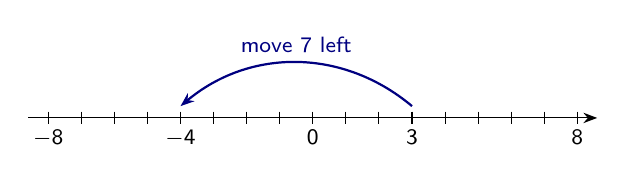
\begin{tikzpicture}[x=0.42cm]
  \draw[-{Stealth[length=5pt]}] (-8.6,0) -- (8.6,0);
  \foreach \n in {-8,...,8} \draw (\n,0.08) -- (\n,-0.08);
  \foreach \n in {-8,-4,0,3,8}
    \node[below,font=\footnotesize,inner sep=2pt] at (\n,-0.08) {$\n$};
  \draw[-{Stealth[length=5pt]},thick,blue!50!black]
    (3,0.15) to[bend right=40] node[above,font=\footnotesize] {move $7$ left} (-4,0.15);
\end{tikzpicture}

So $3-7=-4$, and in the same way $-5+2=-3$.
\end{wexnote}
\end{wex}

\instruction{Fill in the gaps.}

\begin{scaffold}
\ealgloss{Simplify}{Uprość} $4m-3n-9m+n$.

The \ealgloss{like terms}{wyrazy podobne} are $+4m$ and $-9m$, and \gap\ and \gap.

$4m-9m=$ \gap

$-3n+n=$ \gap

So $4m-3n-9m+n=$ \wgap.
\end{scaffold}\hfill
\begin{scaffold}
\ealgloss{Simplify}{Uprość} $p+2q-6p-8q$.

The \ealgloss{like terms}{wyrazy podobne} are \gap\ and \gap, and \gap\ and \gap.

\wgap\ $=$ \gap

\wgap\ $=$ \gap

So $p+2q-6p-8q=$ \wgap.
\end{scaffold}

\instruction{\ealgloss{Simplify}{Uprość}.}

\begin{questions}
\sq{2a-5a}
\sq{4x-9x}
\sq{3c-8c}
\sq{y-6y}
\sq{-3b+b}
\sq{-2m-4m}
\sq{-4y-y}
\sq{-7p+3p}
\sq{-k-k}
\sq{-6n+2n-3n}
\sq{5-2n-9}
\sq{3a+2b-7a}
\sq{2a-3b-5a+b}
\sq{5x-3y-8x+y}
\sql{-4p+6q+p-9q}
\sq{2-5k-7+3k}
\sql{-a-b-2a+4b}
\sq{4c-3-6c-2}
\sql{3xy-5x-7xy+2x}
\sql{8-2c-11-4c+6c}
\end{questions}

\newpage

\topic{6. Multiplying \ealgloss{terms}{wyrazy}}

\begin{wex}
\begin{working}
\ealgloss{Simplify}{Uprość} $3a\times 4b$.

$3a\times 4b=3\times 4\times a\times b$

The numbers: $3\times 4=12$.

The \ealgloss{variables}{zmienne}: $a\times b=ab$.

So $3a\times 4b=12ab$.
\end{working}
\begin{wexnote}
$3a$ means $3\times a$, and $4b$ means $4\times b$.

We can multiply in any order, so we multiply the numbers together and the
\ealgloss{variables}{zmienne} together.

We write the number first, then the \ealgloss{variables}{zmienne} in alphabetical order, with
no $\times$ \ealgloss{signs}{znaki}: $b\times a$ is written $ab$.
\end{wexnote}
\end{wex}

\instruction{Fill in the gaps.}

\begin{scaffold}
\ealgloss{Simplify}{Uprość} $2x\times 5y$.

$2x\times 5y=2\times 5\times x\times y$

The numbers: $2\times 5=$ \gap.

The \ealgloss{variables}{zmienne}: $x\times y=$ \gap.

So $2x\times 5y=$ \gap.
\end{scaffold}\hfill
\begin{scaffold}
\ealgloss{Simplify}{Uprość} $4n\times 3m$.

$4n\times 3m=$ \lgap

The numbers: \gap\ $=$ \gap.

The \ealgloss{variables}{zmienne}: \gap\ $=$ \gap.

So $4n\times 3m=$ \gap.
\end{scaffold}

\instruction{\ealgloss{Simplify}{Uprość}.}

\begin{questions}
\sq{4\times a}
\sq{a\times b}
\sq{3\times 2b}
\sq{5\times 4c}
\sq{y\times x}
\sq{5x\times 2}
\sq{b\times 7}
\sq{2a\times b}
\sq{3x\times y}
\sq{p\times 6q}
\sq{3p\times 4q}
\sq{6x\times 5y}
\sq{4a\times 4b}
\sq{2b\times 9a}
\sq{3n\times 8m}
\sq{7m\times 7n}
\sq{5t\times 4s}
\sq{10x\times 3y}
\sq{4\times 2a\times b}
\sq{2a\times 3b\times c}
\sq{a\times 2b\times 3c}
\sq{4x\times 3yz}
\sq{2xy\times 5z}
\sq{3c\times 2b\times 5a}
\end{questions}

\newpage

\topic{7. Multiplying with \ealgloss{negative}{ujemne} numbers}

\begin{wex}
\begin{working}
\ealgloss{Simplify}{Uprość} $-2x\times -4y$.

$-2x\times -4y=-2\times -4\times x\times y$

The numbers: $-2\times -4=8$.

The \ealgloss{variables}{zmienne}: $x\times y=xy$.

So $-2x\times -4y=8xy$.
\end{working}
\begin{wexnote}
When we multiply two numbers with the same \ealgloss{sign}{znak}, the answer is \ealgloss{positive}{liczba dodatnia}.
When the \ealgloss{signs}{znaki} are different, the answer is \ealgloss{negative}{ujemna}.

\vspace{2pt}
\begin{tabular}{@{}l@{\qquad}l@{}}
$3\times 4=12$     & $-3\times 4=-12$\\[2pt]
$-3\times -4=12$   & $3\times -4=-12$
\end{tabular}

$-a$ means $-1\times a$, so the \ealgloss{coefficient}{współczynnik} of $-a$ is $-1$.
\end{wexnote}
\end{wex}

\instruction{Fill in the gaps.}

\begin{scaffold}
\ealgloss{Simplify}{Uprość} $-3a\times 5b$.

$-3a\times 5b=-3\times 5\times a\times b$

The numbers: $-3\times 5=$ \gap.

The \ealgloss{variables}{zmienne}: $a\times b=$ \gap.

So $-3a\times 5b=$ \gap.
\end{scaffold}\hfill
\begin{scaffold}
\ealgloss{Simplify}{Uprość} $6m\times -2n$.

$6m\times -2n=$ \lgap

The numbers: \gap\ $=$ \gap.

The \ealgloss{variables}{zmienne}: \gap\ $=$ \gap.

So $6m\times -2n=$ \gap.
\end{scaffold}

\instruction{\ealgloss{Simplify}{Uprość}.}

\begin{questions}
\sq{-2\times 3a}
\sq{-5\times 2y}
\sq{4\times -5b}
\sq{-3\times -2x}
\sq{-6\times -3c}
\sq{-8\times -k}
\sq{-a\times b}
\sq{a\times -b}
\sq{-x\times -y}
\sq{5p\times -2q}
\sq{-4a\times 3b}
\sq{-3m\times 4n}
\sq{-6m\times -n}
\sq{-7x\times -3y}
\sq{-2x\times -9y}
\sq{2c\times -9d}
\sq{8p\times -q}
\sq{-5b\times -4a}
\sq{-10a\times -10b}
\sq{-2a\times 3b\times c}
\sq{3x\times -2y\times 4z}
\sq{2x\times -3y\times -z}
\sq{-4p\times -q\times 5r}
\sq{-2a\times -3b\times -c}
\end{questions}

\newpage

\topic{8. \ealgloss{Squares}{kwadraty} and \ealgloss{cubes}{sześciany}}

\begin{wex}
\begin{working}
\ealgloss{Simplify}{Uprość} $3a\times 2a$.

$3a\times 2a=3\times 2\times a\times a$

The numbers: $3\times 2=6$.

The \ealgloss{variables}{zmienne}: $a\times a=a^2$.

So $3a\times 2a=6a^2$.
\end{working}
\begin{wexnote}
$a\times a$ is written $a^2$, which we say as ``$a$ \ealgloss{squared}{kwadrat}''.
$a\times a\times a$ is written $a^3$, which we say as ``$a$ \ealgloss{cubed}{sześcian}''.

The small number is called the \ealgloss{index}{wykładnik}. It tells us how many times
the \ealgloss{variable}{zmienna} is multiplied: $a^4=a\times a\times a\times a$.

$a^2b$ means $a\times a\times b$.
\end{wexnote}
\end{wex}

\instruction{Fill in the gaps.}

\begin{scaffold}
\ealgloss{Simplify}{Uprość} $5x\times 4x$.

$5x\times 4x=5\times 4\times x\times x$

The numbers: $5\times 4=$ \gap.

The \ealgloss{variables}{zmienne}: $x\times x=$ \gap.

So $5x\times 4x=$ \gap.
\end{scaffold}\hfill
\begin{scaffold}
\ealgloss{Simplify}{Uprość} $2y\times 3y\times y$.

$2y\times 3y\times y=$ \lgap

The numbers: \gap\ $=$ \gap.

The \ealgloss{variables}{zmienne}: \wgap\ $=$ \gap.

So $2y\times 3y\times y=$ \gap.
\end{scaffold}

\instruction{\ealgloss{Simplify}{Uprość}.}

\begin{questions}
\sq{b\times b}
\sq{y\times y}
\sq{x\times x\times x}
\sq{m\times m\times m\times m}
\sq{3\times a\times a}
\sq{5\times c\times c}
\sq{2p\times p}
\sq{3q\times q}
\sq{a\times 6a}
\sq{4y\times 3y}
\sq{7a\times 2a}
\sq{5k\times 5k}
\sq{9h\times 9h}
\sq{6t\times t\times t}
\sq{2n\times 3n\times 4n}
\sq{-p\times p}
\sq{-3x\times 4x}
\sq{-5x\times -x}
\sq{-2y\times -5y}
\sq{3d\times 2d\times d\times d}
\sq{-4c\times -c\times 2c}
\sq{a\times a\times b}
\sq{x\times y\times y}
\sq{p\times p\times q\times q}
\end{questions}

\newpage

\topic{9. Multiplying \ealgloss{powers}{potęgi}}

\begin{wex}
\begin{working}
\ealgloss{Simplify}{Uprość} $2a^3\times 4a^2$.

$2a^3\times 4a^2=2\times 4\times a^3\times a^2$

The numbers: $2\times 4=8$.

The \ealgloss{variables}{zmienne}:

$a^3\times a^2=a^{3+2}=a^5$

So $2a^3\times 4a^2=8a^5$.
\end{working}
\begin{wexnote}
$a^3\times a^2=\underbrace{a\times a\times a}_{a^3}\times
  \underbrace{a\times a}_{a^2}=a^5$

When we multiply \ealgloss{powers}{potęgi} of the same \ealgloss{variable}{zmienna}, we add the \ealgloss{indices}{wykładniki}:
$3+2=5$.

A \ealgloss{variable}{zmienna} with no \ealgloss{index}{wykładnik} has an \ealgloss{index}{wykładnik} of $1$: $a=a^1$. So
$a^4\times a=a^{4+1}=a^5$.
\end{wexnote}
\end{wex}

\instruction{Fill in the gaps.}

\begin{scaffold}
\ealgloss{Simplify}{Uprość} $3x^4\times 5x^2$.

$3x^4\times 5x^2=3\times 5\times x^4\times x^2$

The numbers: $3\times 5=$ \gap.

The \ealgloss{variables}{zmienne}:

$x^4\times x^2=x^{4+2}=$ \gap

So $3x^4\times 5x^2=$ \gap.
\end{scaffold}\hfill
\begin{scaffold}
\ealgloss{Simplify}{Uprość} $6y^5\times 2y$.

$6y^5\times 2y=$ \lgap

The numbers: \gap\ $=$ \gap.

The \ealgloss{variables}{zmienne}:

\gap\ $=y^{\boxgap+\boxgap}=$ \gap

So $6y^5\times 2y=$ \gap.
\end{scaffold}

\instruction{\ealgloss{Simplify}{Uprość}.}

\begin{questions}
\sq{a^2\times a^3}
\sq{x^4\times x^5}
\sq{p^2\times p^2}
\sq{n^3\times n^3}
\sq{z^7\times z^2}
\sq{b^3\times b}
\sq{m\times m^6}
\sq{q\times q^4}
\sq{y^{10}\times y^3}
\sq{2a^2\times 3a^4}
\sq{5x^3\times 2x^3}
\sq{4b^2\times 5b^2}
\sq{6x^2\times 3x^3}
\sq{4y\times 3y^2}
\sq{2m^5\times m}
\sq{k^2\times 7k^5}
\sq{c^2\times c^3\times c}
\sq{h^4\times h\times h^2}
\sq{-2a^5\times 3a^2}
\sq{6n^4\times -n^4}
\sq{-y^2\times -y^3}
\sq{-4t^3\times -5t^6}
\sq{3d^2\times 2d\times d^4}
\sq{-2x^3\times -3x^2\times -x}
\end{questions}

\newpage

\topic{10. Multiplying \ealgloss{terms}{wyrazy} with more than one \ealgloss{variable}{zmienna}}

\begin{wex}
\begin{working}
\ealgloss{Simplify}{Uprość} $3a^2b\times 2ab^3$.

$3a^2b\times 2ab^3$\\
\hspace*{1em}$=3\times 2\times a^2\times a\times b\times b^3$

The numbers: $3\times 2=6$.

The \ealgloss{powers}{potęgi} of $a$: $a^2\times a=a^3$.

The \ealgloss{powers}{potęgi} of $b$: $b\times b^3=b^4$.

So $3a^2b\times 2ab^3=6a^3b^4$.
\end{working}
\begin{wexnote}
$a^2b$ means $a^2\times b$, and $ab^3$ means $a\times b^3$.

We multiply the numbers, and then we multiply the \ealgloss{powers}{potęgi} of each \ealgloss{variable}{zmienna}
separately. We add the \ealgloss{indices}{wykładniki} of $a$, and then we add the \ealgloss{indices}{wykładniki} of
$b$.

We do not add the \ealgloss{indices}{wykładniki} of different \ealgloss{variables}{zmienne}: $a^3\times b^4$ is
written $a^3b^4$.
\end{wexnote}
\end{wex}

\instruction{Fill in the gaps.}

\begin{scaffold}
\ealgloss{Simplify}{Uprość} $4x^3y\times 2xy^2$.

$4x^3y\times 2xy^2$\\
\hspace*{1em}$=4\times 2\times x^3\times x\times y\times y^2$

The numbers: $4\times 2=$ \gap.

The \ealgloss{powers}{potęgi} of $x$: $x^3\times x=$ \gap.

The \ealgloss{powers}{potęgi} of $y$: $y\times y^2=$ \gap.

So $4x^3y\times 2xy^2=$ \wgap.
\end{scaffold}\hfill
\begin{scaffold}
\ealgloss{Simplify}{Uprość} $5m^2n^3\times 3mn^4$.

$5m^2n^3\times 3mn^4$\\
\hspace*{1em}$=$ \lgap

The numbers: \gap\ $=$ \gap.

The \ealgloss{powers}{potęgi} of $m$: \gap\ $=$ \gap.

The \ealgloss{powers}{potęgi} of $n$: \gap\ $=$ \gap.

So $5m^2n^3\times 3mn^4=$ \wgap.
\end{scaffold}

\instruction{\ealgloss{Simplify}{Uprość}.}

\begin{questions}
\sq{a^2b\times a}
\sq{x\times xy}
\sq{y\times xy}
\sq{ab\times ab}
\sq{2a\times 3ab}
\sq{4m\times 2mn}
\sq{3m^2\times 4n}
\sq{p^2q\times pq}
\sq{x^2y\times xy^3}
\sq{pq^2\times p^2q}
\sq{2ab\times 3bc}
\sq{2a^2b\times 3ab}
\sq{4m^2n\times 2mn^2}
\sq{-3pq\times 2q}
\sq{5x^2y^3\times x^4y}
\sq{4x^2y\times -3xy}
\sq{-3a^3b^2\times 2ab}
\sq{5xy^2\times -2x^3y}
\sq{3p^2q\times 2pq\times q^2}
\sq{-2a^2b^3\times -5a^4b}
\end{questions}

\newpage

\topic{11. \ealgloss{Collecting}{redukowanie} \ealgloss{like terms}{wyrazy podobne} with \ealgloss{powers}{potęgi}}

\begin{wex}
\begin{working}
\ealgloss{Simplify}{Uprość} $5a^2+3a-2a^2+4a$.

The \ealgloss{like terms}{wyrazy podobne} are $+5a^2$ and $-2a^2$, and $+3a$ and $+4a$.

$5a^2-2a^2=3a^2$

$3a+4a=7a$

So $5a^2+3a-2a^2+4a=3a^2+7a$.
\end{working}
\begin{wexnote}
\ealgloss{Like terms}{wyrazy podobne} have exactly the same \ealgloss{variables}{zmienne}, with the same \ealgloss{indices}{wykładniki}.
$5a^2$ and $-2a^2$ are \ealgloss{like terms}{wyrazy podobne}. $5a^2$ and $3a$ are not \ealgloss{like terms}{wyrazy podobne},
because $a^2=a\times a$ is not the same as $a$.

When we \ealgloss{collect}{redukujemy} \ealgloss{like terms}{wyrazy podobne}, we add the \ealgloss{coefficients}{współczynniki} and the \ealgloss{index}{wykładnik} stays
the same: $a^2+a^2=2a^2$.

$a^2b$ and $ab^2$ are not \ealgloss{like terms}{wyrazy podobne}.
\end{wexnote}
\end{wex}

\instruction{Fill in the gaps.}

\begin{scaffold}
\ealgloss{Simplify}{Uprość} $4x^2+6x+x^2-2x$.

The \ealgloss{like terms}{wyrazy podobne} are $+4x^2$ and $+x^2$, and \gap\ and \gap.

$4x^2+x^2=$ \gap

$6x-2x=$ \gap

So $4x^2+6x+x^2-2x=$ \wgap.
\end{scaffold}\hfill
\begin{scaffold}
\ealgloss{Simplify}{Uprość} $7y^2-5y-y^2+y$.

The \ealgloss{like terms}{wyrazy podobne} are \gap\ and \gap, and \gap\ and \gap.

\wgap\ $=$ \gap

\wgap\ $=$ \gap

So $7y^2-5y-y^2+y=$ \wgap.
\end{scaffold}

\instruction{\ealgloss{Simplify}{Uprość}. If an \ealgloss{expression}{wyrażenie} cannot be \ealgloss{simplified}{uprościć}, write
``cannot be \ealgloss{simplified}{uprościć}''.}

\begin{questions}
\sq{3a^2+4a^2}
\sq{6x^3-2x^3}
\sq{9b^2-b^2}
\sq{y^2+y^2}
\sq{4c^2-c^2+2c}
\sq{5b^2+2b+b^2}
\sq{4y^2+3y+2y}
\sq{p^2+p+p^2+p}
\sq{2a^2-5a^2}
\sql{7a^2-3a-2a^2+5a}
\sql{x^2+3x-4x^2-5x}
\sql{3m^3+2m^2+m^3-m^2}
\sq{a^2+a+1}
\sql{4ab+3a^2-ab+a^2}
\sql{5k^2-3k+2-2k^2+k-7}
\sql{2x^2y+3xy^2+5x^2y}
\sql{6c^3-c^2+4c-2c^3+3c^2}
\sql{a^2b-4ab^2+3a^2b+ab^2}
\end{questions}

\newpage

\topic{12. Multiplying and \ealgloss{collecting}{redukowanie} \ealgloss{like terms}{wyrazy podobne}}

\begin{wex}
\begin{working}
\ealgloss{Simplify}{Uprość} $2a\times 3a+4a^2$.

We multiply first:

$2a\times 3a=6a^2$

So $2a\times 3a+4a^2=6a^2+4a^2$.

We \ealgloss{collect}{redukujemy} the \ealgloss{like terms}{wyrazy podobne}:

$6a^2+4a^2=10a^2$

So $2a\times 3a+4a^2=10a^2$.
\end{working}
\begin{wexnote}
We multiply before we add or subtract, in the same way as
$2\times 3+4=6+4=10$.

After we multiply, we write each \ealgloss{term}{wyraz} with the number first and the
\ealgloss{variables}{zmienne} in alphabetical order. Then we can see which \ealgloss{terms}{wyrazy} are \ealgloss{like terms}{wyrazy podobne}: $3y\times 2x=6xy$, which is a \ealgloss{like term}{wyraz podobny} with $xy$.
\end{wexnote}
\end{wex}

\instruction{Fill in the gaps.}

\begin{scaffold}
\ealgloss{Simplify}{Uprość} $3x\times 2y+5xy$.

We multiply first:

$3x\times 2y=$ \gap

So $3x\times 2y+5xy=$ \gap\ $+\,5xy$.

We \ealgloss{collect}{redukujemy} the \ealgloss{like terms}{wyrazy podobne}:

\gap\ $+\,5xy=$ \gap

So $3x\times 2y+5xy=$ \gap.
\end{scaffold}\hfill
\begin{scaffold}
\ealgloss{Simplify}{Uprość} $4m\times m-m^2$.

We multiply first:

\wgap\ $=$ \gap

So $4m\times m-m^2=$ \wgap.

We \ealgloss{collect}{redukujemy} the \ealgloss{like terms}{wyrazy podobne}:

\wgap\ $=$ \gap

So $4m\times m-m^2=$ \gap.
\end{scaffold}

\instruction{\ealgloss{Simplify}{Uprość}.}

\begin{questions}
\sq{2a\times 4b+3ab}
\sq{5x\times x+2x^2}
\sq{3p\times 2q-pq}
\sq{a^2\times a+4a^3}
\sq{6y^2-2y\times y}
\sq{7mn+2m\times 3n}
\sql{2a\times 3b+4a\times b}
\sql{3x\times 2x-x\times 5x}
\sql{2m^2\times 3m+m^3}
\sq{4a\times 2a+3a}
\sql{5x\times 2y-3y\times 4x}
\sql{ab\times ab+3a^2b^2}
\sql{-3k\times 2k+k^2+4k}
\sql{2a\times 3a^2+4a\times a\times a}
\sql{3p^2\times 2p^3-4p\times p^4}
\sql{2x\times 3y+4x\times 5x-xy}
\end{questions}

\newpage

\topic{13. Problem solving}

\instruction{Write the missing \ealgloss{term}{wyraz} in the box.}

\begin{multicols}{2}
\qlabel$3a\times{}$\missing${}=12ab$\par\vspace{12pt}
\qlabel$5y+{}$\missing${}=8y$\par\vspace{12pt}
\qlabel\missing${}\times 2x^2=10x^5$\par\vspace{12pt}
\qlabel$4p+{}$\missing${}-2p=2p+3q$\par\vspace{12pt}
\qlabel\missing${}\times -3y=6xy$\par\vspace{12pt}
\qlabel$5a^2+{}$\missing${}=2a^2$\par\vspace{12pt}
\qlabel$2m^3\times{}$\missing${}=8m^7n$\par\vspace{12pt}
\qlabel$2c+5d+4c+{}$\missing${}=5d$\par
\end{multicols}

\vspace{10pt}
\qlabel Sam \ealgloss{simplifies}{upraszcza} $2a+3b$ and writes $5ab$. Explain the mistake that
Sam has made.
\writeline\writeline

\vspace{10pt}
\qlabel Priya says that $a^2+a^3=a^5$. Is Priya right? Explain your answer.
\writeline\writeline

\vspace{10pt}
\qlabel Tom says that $3a\times 4a=12a$. Explain the mistake that Tom has
made, and write the correct answer.
\writeline\writeline

\vspace{10pt}
\begin{minipage}[t]{0.58\linewidth}
\raggedright
\qlabel The \ealgloss{rectangle}{prostokąt} has length $5x$ and width $2y$.\par
\leftskip=\qlabelwidth
\vspace{6pt}
(a) Write a \ealgloss{simplified}{uproszczone} \ealgloss{expression}{wyrażenie} for the \ealgloss{perimeter}{obwód} of the \ealgloss{rectangle}{prostokąta}.
\writeline

\vspace{6pt}
(b) Write a \ealgloss{simplified}{uproszczone} \ealgloss{expression}{wyrażenie} for the \ealgloss{area}{pole} of the \ealgloss{rectangle}{prostokąta}.
\writeline
\end{minipage}\hfill
\begin{minipage}[t]{0.38\linewidth}
\centering
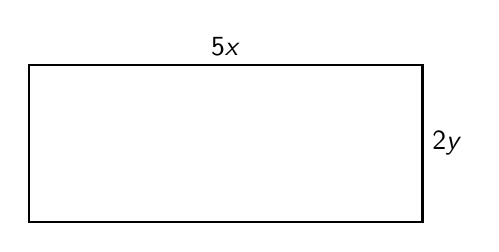
\begin{tikzpicture}[baseline=(current bounding box.north)]
  \draw[thick] (0,0) rectangle (5,2);
  \node[above] at (2.5,2) {$5x$};
  \node[right] at (5,1) {$2y$};
\end{tikzpicture}
\end{minipage}

\vspace{14pt}
\qlabel The \ealgloss{area}{pole} of a \ealgloss{rectangle}{prostokąta} is $12a^2$. Write down three different pairs
of lengths that its sides could have.
\writeline\writeline

\vspace{10pt}
\qlabel Write an \ealgloss{expression}{wyrażenie} with four \ealgloss{terms}{wyrazy} that \ealgloss{simplifies}{upraszcza} to $5x-2y$.
\writeline

\vspace{10pt}
\qlabel Write three different multiplications that \ealgloss{simplify}{uprościć} to $6a^2b$.
\writeline

\end{ealglossed}
\end{document}